%!TEX root = ACC2019.tex

\begin{section}{Approach}
\label{sec:approach}
In this section we describe the framework for detection of sensor attacks for systems with unknown or changing dynamics and adaptive motion planning to solve Problems \ref{problem1} and \ref{problem2} and ensure vehicle's safety. We follow the architecture in the block diagram of Fig. \ref{fig:system_arch} to solve these problems. A detector monitors multiple input measurements for sensor attacks, which allows an uncompromised input $u(k)$ to control the system. At the same time, the state estimator along with the high level motion planner update the reference $r(k)$ of the controller to ensure safety. 

\begin{figure}[th!]
\vspace{5pt}
\centering
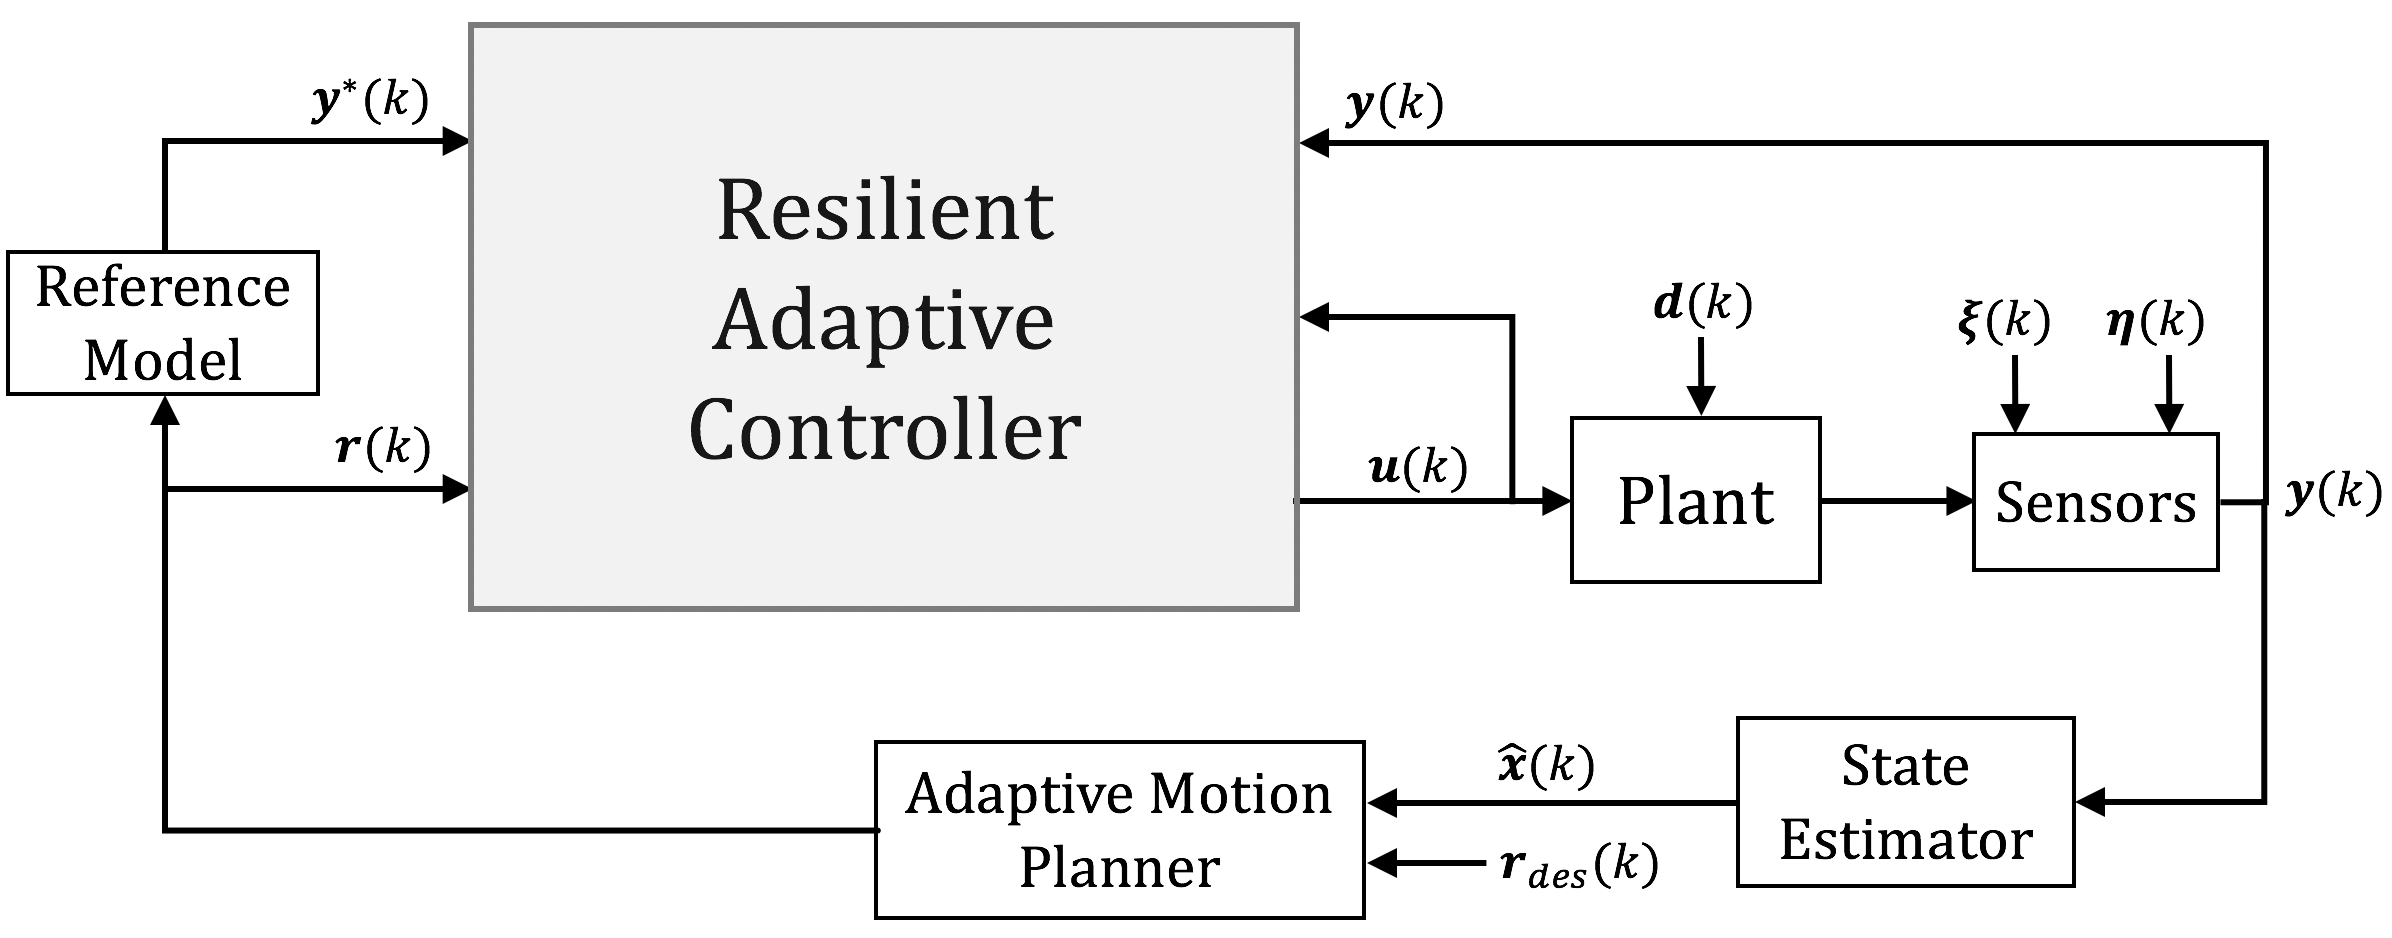
\includegraphics[width=0.46\textwidth]{Figures/sys_arch.png}
\vspace{-2pt}
\caption{Overall system architecture showing the relationship between the reference model adaptive controller and the adaptive motion planner.}
\label{fig:system_arch}
\vspace{-12pt}
\end{figure}
% \NB{FIGURE: where is the adaptive controller? Group blocks together that represent the Resilient AC.}
% \NB{FIGURE: we need to have multiple arrows going out from the controller}
% \NB{FIGURE: name the motion planner differently like adaptive motion planner}
Next, we describe the framework for attack detection and sensor reconfiguration using a series of adaptive controlled subsystems.

\subsection{Resilient Adaptive Control}
\label{sec:Res_adapt_control}


In order to detect and remove attacks we propose the architecture in Fig. \ref{fig:det_arch} in which redundant sensor measurements are considered. Specifically, multiple subsystems are considered, one for each sensor measurement and within each subsystem a model reference adaptive control scheme is implemented to obtain the desired input $u^*$ to track a reference signal $y^*$. As in our previous work \cite{6943080,7879899} we assume that less than $s/2$ sensors can be compromised in order to estimate the state of the system.


% The architecture followed in this work is shown in Fig. \ref{fig:det_arch}, which consists of a subsystem for each sensor measurement within the same controlled state. Each subsystem consists of a model reference adaptive controller to generate the next input $u^*_i$ where $i=1,2,\dots,s$ given its corresponding measurement signal $y_i$.

\begin{figure}[h!]
\vspace{-3pt}
\centering
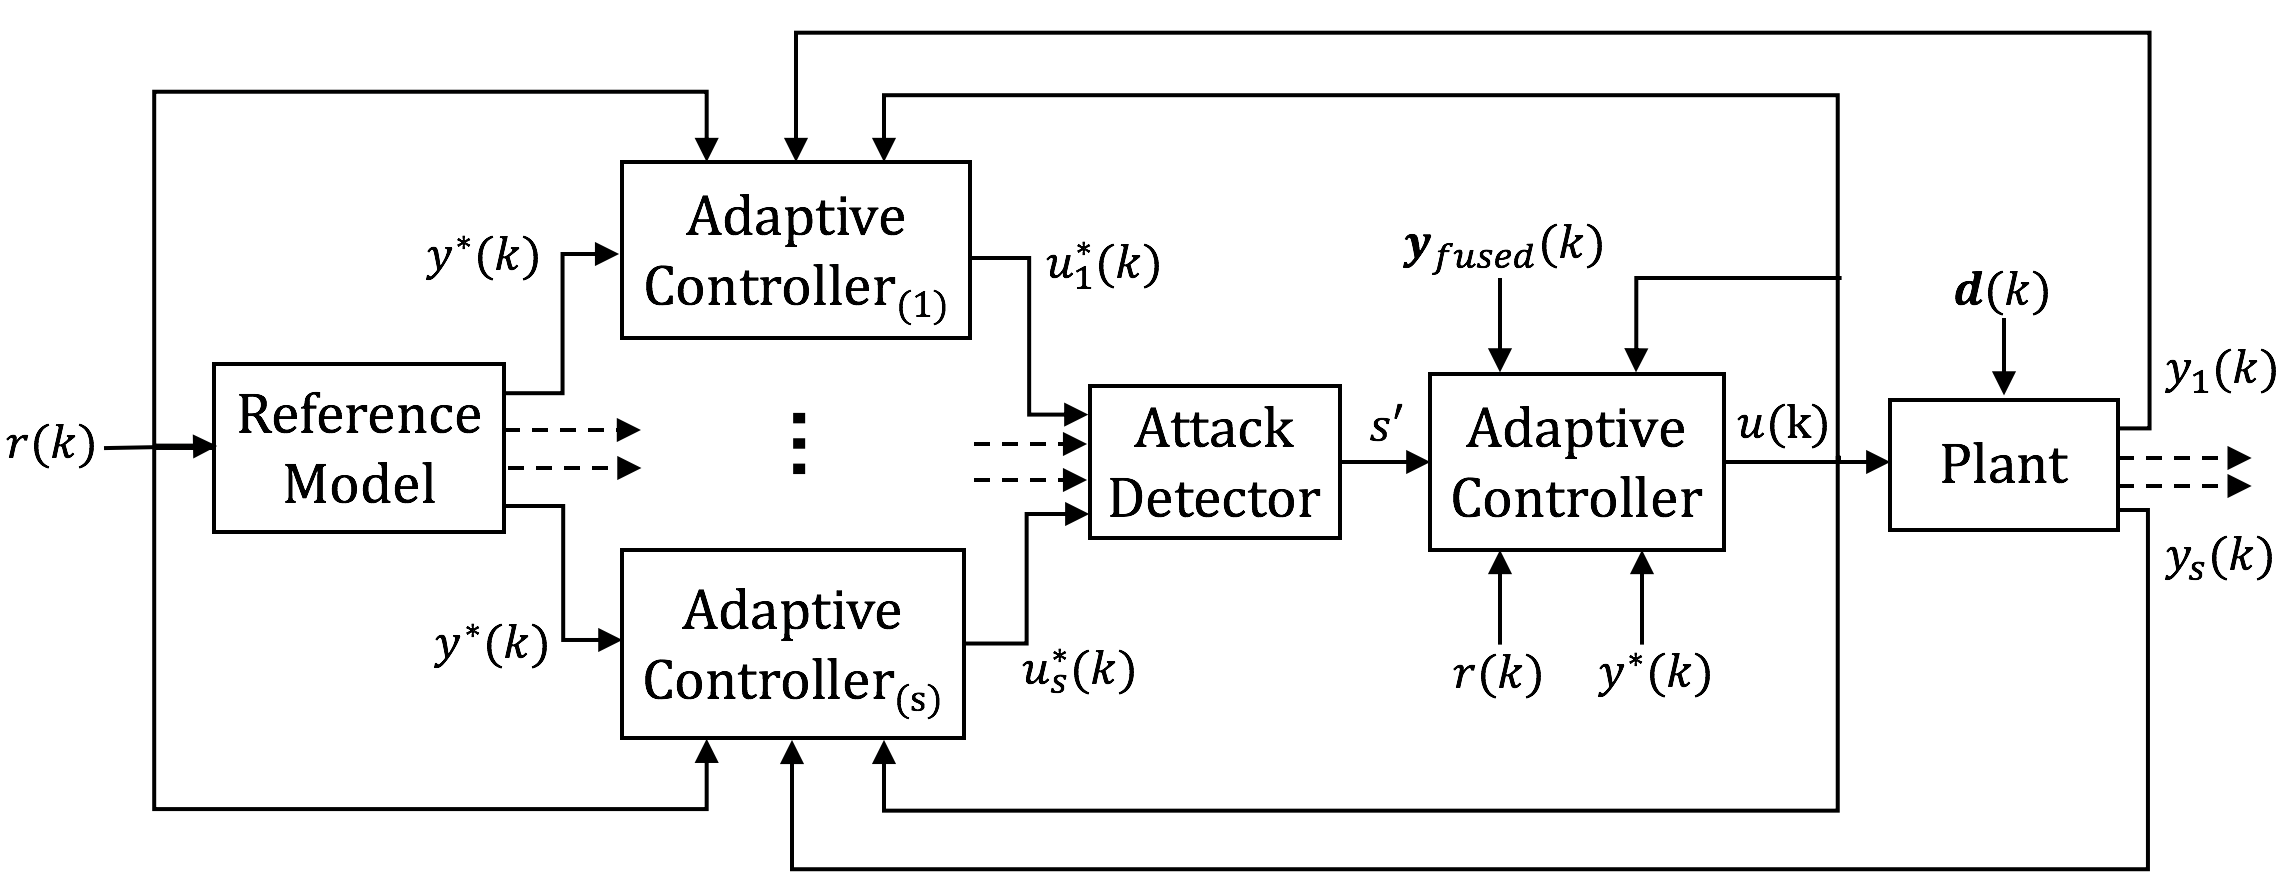
\includegraphics[width=0.48\textwidth]{Figures/con_and_det.png}
\caption{Architecture of the Resilient Adaptive Controller (RAC) detection scheme within the $s$ associated with each sensor measurement. }
\label{fig:det_arch}
\end{figure}
%\eqref{eq:Start}$-$\eqref{eq:End}

First, to design the resilient model reference adaptive controller, we assume that:
	\begin{enumerate}%[leftmargin=3\parindent]
%	\item[$A1)$] all zeros of $B^{'}(z^{-1})z^q$ from \eqref{eq:B_prime} are within $|z|<1$. 
	\item[$A1)$] all numerator zeros of \eqref{eq:transfer_function} are within $|z|<1$.
	\item[$A2)$] $p$ and $q$ are known. 
	\item[$A3)$] the system delay $d$ is known.
	\item[$A4)$] all poles of $E(z^{-1})z^w$ from \eqref{eq:reference model_z} are within $|z|<1$, where $w$ is the order of $E(z^{-1})$.
	\end{enumerate}
The zeros $z$ of the system are within the $z-plane$ while $p$, $q$, and $d$ are the dimensions of \eqref{eq:transfer_function}. With these assumptions satisfied, every $i^{th}$ subsystem can generate an input signal $u^*_i(k)$ to have its measurement signal $y_i$ track a given tracking signal $y^*$ from the reference model \eqref{eq:reference model_z}. Many of the steps to design the CMBAC Model Reference Adaptive Controller (MRAC) are omitted here, but can be found in \cite{tao2003adaptive}. In what follows, we provide the main equations to compute the desired input when dealing with changing systems. 
% The model in \eqref{eq:discrete_SS} can be transformed in a discrete-time transfer function form which is a usable form for the resilient adaptive control approach later in \ref{sec:Res_adapt_control}. To solve Problem 1 and detect cyber-attacks while adapting the system, we leverage the CMBAC adaptive control approach presented in \cite{4106038}, in which the objective is to compute an input to have the system follow a reference model given changing dynamics (i.e. dynamic $\bm{A_d}$ and  $\bm{B_d}$). Here we summarize the model which will be used later in Section \ref{sec:Res_adapt_control} to adapt the system under uncertainties and to detect attacks. 
% The state space model in a \eqref{eq:discritzed_SS_model} transformed in discrete-time transfer function, in single-input single-output (SISO) form, within the $z$-domain becomes:
% 	\begin{equation}
% 	\begin{split}
% 	\label{eq:transfer_function}
%         G(z) & = \frac{y(z)}{u(z)} = \bm{C}(z\bm{I}-\bm{A}_d)^{-1}\bm{B}_d  \\
% 	& = \frac{b_0z^{p-d}+b_1z^{p-d-1} +...+b_qz^{p-d-q}}{z^{p}+a_1z^{p-1}+...+a_{p-1}z+a_p} 
% 	\end{split}
% 	\end{equation}
% with $b_0\ne{0}$, $d>0$, $p-d-q\geq{0}$, $p$ and $q$ are orders of the denominator and numerator, and $d$ is the system delay. A reference model of desired characteristics is chosen for the system in \eqref{eq:transfer_function} to follow, which can be expressed as:
% 	\begin{equation}
% 	\label{eq:reference model_z}
% 	\frac{y^*(z)}{r(z)}=\frac{z^{-d}gH(z^{-1})}{E(z^{-1})}
% 	\end{equation}
% 	where $g$ is a constant to ensure a 1:1 steady state ratio of the reference $r$ and tracking signal $y^*$. 
A parameter vector of unknown coefficients describing the system's transfer function \eqref{eq:transfer_function} to follow the desired reference model is described as:
    \begin{equation}
	\bm{\theta}_0=(\alpha_0, \dots ,\alpha_{p-1},\beta_0, \dots ,\beta_{q+d-1})^T \in \R^{p+q+d}
	\end{equation}
The objective of the adaptive control is to estimate the true parameters of $\bm{\theta}_0$ with the parameter estimate vector $\bm{\theta}(k)$:
    \begin{equation}
    \bm{\theta}(k)=(\theta_1(k), \dots ,\theta_p(k),\theta_{p+1}(k), \dots ,\theta_{p+q+d}(k))^T
	\end{equation}
With our known input and measurement signals within a signal vector $\bm{\phi}(k)$,
	\begin{equation}
	\begin{split}
	\bm{\phi}(k)&=(y_i(k), \dots ,y_i(k-p+1),u^*_i(k), \dots , \\
	& u^*_i(k-q-d+1))^T \in \R^{p+q+d}
	\end{split}
	\end{equation}
we can estimate the true parameter vector $\bm{\theta}_0$ by updating $\bm{\theta}(k)$ using a \textit{Modified Projection Algorithm} \cite{tao2003adaptive}:
	\begin{equation}
	\label{eq:Modified_Proj_Algorithm}
	\bm{\theta}(k)=\bm{\theta}(k-1)+\frac{a(k)\bm{\phi}(k-d)e(k)}{c+\bm{\phi}^T(k-d)\bm{\phi}(k-d)}
	\end{equation}
% 	\begin{equation}
% 	e(k)=E(z^{-1})y_i(k)-\theta^T(k-1)\bm{\phi}(k-d)
% 	\end{equation}
where $e(k)$ is the estimation error, $\epsilon<a(k)<2-\epsilon$, $\epsilon<1$ and $c>0$. To follow the desired tracking output $y^*(k)$ from the reference model, the adaptive control input $u^*_i(k)$ is then calculated from the equation:
%     \begin{equation}
%     \label{eq:tracking_model}
% 	\bm{\theta}^T(k)\bm{\phi}(k)=E(z^{-1})y^*(k+d)
% 	\end{equation}
% By rearranging \eqref{eq:tracking_model} we isolate $u^*_i(k)$ to calculate our next input signal for each $i^{th}$ subsystem for $i=1,\dots,s$:
	\begin{equation}
	\begin{split}
	\label{eq:End}
	u^*_i(k)&=\frac{1}{\theta_{p+1}(k)}\big(-\theta_1(k)y_i(k)-\theta_2(k)y_i(k-1)  \\
    -\dots &-\theta_p(k)y_i(k-p-1)-\theta_{p+2}(k)u^*_i(k-1)  \\
	- \dots &- \theta_{p+q+d}(k)u^*_i(k-q-d+1) + y^*(k)) \big)^T
	\end{split}
	\end{equation}
where $\theta_{p+1}(k)\neq0 $. Once these subsystem inputs are computed, under the assumptions in (A1-A4) we leverage the following MRAC properties to detect sensor attacks when the system model has changed. In \cite{tao2003adaptive}, the following properties are found to be true when implementing an MRAC,
	\begin{enumerate}%[label=(\roman*),leftmargin=4\parindent]
	\label{assumtions_ensure}
	\item[$T1)$] $y(k)$ and $u(k)$ are bounded 
	\item[$T2)$] $\lim_{k\to\infty}(y(k)-y^*(k))=0$
	\label{Truth2}
	\item[$T3)$] $\sum_{k=0}^\infty(y(k)-y^*(k))^2<\infty$
	\end{enumerate}
where $y(k)$ is the system output and $y^*(k)$ is a tracking signal from the reference model. These properties ensure that the system's output asymptotically converges to the reference model's tracking signal in a finite amount of time. 


The resilient adaptive controller employs the architecture of redundant subsystems where each sensor measurement $y_i$ has its adaptive controller to generate an input $u^*_i$ to follow a desired tracking signal $y^*_i$. Each of the sensor measurements, when uncompromised, have convergence (T2) towards their desired tracking signal from the corresponding reference model,
    \begin{equation}
    \label{multiple_output_tracking}
    \lim_{k\to\infty}(y_i(k)-y^*_i(k))=0, \;\;\; i=1,\dots,s
    \end{equation}
Since \eqref{multiple_output_tracking} should hold during any operation (e.g., changing dynamics, disturbances) the following equation is also true:
\begin{equation}
    \label{eq:u_to_0}
    \lim_{k\to\infty}(u^*_i(k)-u^*_j(k))=0, \text{ }i\neq j
\end{equation}
where $u^*_i$ and $u^*_j$ refer to inputs calculated from their respected subsystems to track the same signal $y^*(k)$ and $i,j = 1,\dots,s$. Each subsystem input while under ideal conditions (i.e., considering perfect measurements with no noise), should converge to the same value as all other inputs. For each subsystem to compute the next input $u^*_i(k)$, its sensor measurement $y_i$ needs to be uncompromised. As a measurement is corrupted due to a non-zero element from the sensor attack vector, the corresponding subsystem's computed input diverges from the remaining inputs. Mathematically, to detect attacks, a difference matrix $\bm{\Psi}(k)$ is designed for every time interval $k$ of each controlled state. The structure of this matrix is,
    \begin{equation}
    \label{eq:difference_matrix}
	\bm{\Psi}(k)=\begin{bmatrix} \psi_{1,1}(k) & \psi_{1,2}(k) & \dots & \psi_{1,s}(k) \\ \psi_{2,1}(k) & \psi_{2,2}(k) &  &  \\ \vdots &  & \ddots &  \\ \psi_{s,1}(k) &  &  & \psi_{s,s}(k) \end{bmatrix}
	\end{equation}
where $\bm{\Psi}(k) \in \R^{s\times s}$. Each element $\psi_{i,j}\in\bm{\Psi}$ is an error computed as the absolute difference between two subsystem inputs:
    \begin{equation}
        \label{eq:input_diff}
        \psi_{i,j}(k)=|u^*_i(k)-u^*_j(k)|
    \end{equation}
The $l_1$ vector norm for each row in \eqref{eq:difference_matrix} is computed giving the following vector:
    \begin{equation}
    \label{eq:difference_vector}
	\bm{\Psi^{'}}(k)=\begin{bmatrix} \lVert{\bm{\Psi}_1(k)}\rVert_1 \\ \lVert{\bm{\Psi}_2(k)}\rVert_1 \\ \vdots \\ \lVert{\bm{\Psi}_s(k)}\rVert_1 \end{bmatrix}
	\end{equation}

%     \begin{equation}
%     \label{eq:difference_vector}
% 	\bm{\Psi^{'}}(k)=\begin{bmatrix} \lVert{\bm{\Psi}_1(k)}\rVert_1 & \dots & \lVert{\bm{\Psi}_s(k)}\rVert_1 \end{bmatrix}^T
% 	\end{equation}
The minimum value element of \eqref{eq:difference_vector} is used to form another vector $\bm{\Psi}^{'}_{min}(k) \in \R^s$, with every element equal to $\min \bm{\Psi}^{'}(k)$:
%     \begin{equation}
% 	\bm{\Psi}^{'}_{min}(k)=\begin{bmatrix} \min \bm{\Psi}^{'}(k),& \dots \text{ },&\min \bm{\Psi}^{'}(k) \end{bmatrix}^T
% 	\end{equation}
    \begin{equation}
	\bm{\Psi}^{'}_{min}(k)=\min \bm{\Psi}^{'}(k){\bm{1}}_s
	\end{equation}
where ${\bm{1}}_s$ is a $s\times1$ vector of 1's. We can now define the updated error vector as:
    \begin{equation}
    \begin{split}
    \label{eq:Psi2}
	\bm{\Psi}^{''}(k)&=\bm{\Psi}^{'}(k)-\bm{\Psi}^{'}_{min}(k) \\
	&=\begin{bmatrix} \lVert{\bm{\Psi}_1(k)}\rVert_1 - \min \bm{\Psi}^{'}(k)\\ \lVert{\bm{\Psi}_2(k)}\rVert_1 - \min \bm{\Psi}^{'}(k)\\ \vdots \\ \lVert{\bm{\Psi}_s(k)}\rVert_1 - \min \bm{\Psi}^{'}(k) \end{bmatrix}
	\end{split}
	\end{equation}
%     \begin{equation}
%     \label{eq:Psi2}
% 	\bm{\Psi}^{''}(k)=\bm{\Psi}^{'}(k)-\bm{\Psi}^{'}_{min}(k)
% 	\end{equation}
From \eqref{eq:u_to_0} while under ideal conditions (i.e., with no noise), the error vector \eqref{eq:Psi2} has all elements equal to zero. When an $i^{th}$ sensor is under attack, the $i^{th}$ input diverges from the remaining uncompromised inputs. The $i^{th}$ element of $\bm{\Psi}^{''}(k)$ becomes non-zero due to the compromised sensor, while the rest of the elements remain zero. 

Under non-ideal conditions where noises exist, the elements of the error vector will not remain zero while sensors are uncompromised. By setting a threshold value $\delta$, all elements of the error vector need to stay below this level. By refining \eqref{eq:Psi2} for non-ideal conditions we get,
%     \begin{equation}
%     \label{eq:Psi2_nonideal}
% 	\bm{\Psi^{''}}(k)=\bm{\Psi^{'}}(k)-\bm{\Psi}^{'}_{min}(k) \leq \bm{\delta}(k)
% 	\end{equation}
    \begin{equation}
    \begin{split}
    \label{eq:Psi2_nonideal}
	\bm{\Psi}^{''}(k)&=\bm{\Psi}^{'}(k)-\bm{\Psi}^{'}_{min}(k) \\
	&=\begin{bmatrix} \lVert{\bm{\Psi}_1(k)}\rVert_1 - \min \bm{\Psi}^{'}(k)\\ \lVert{\bm{\Psi}_2(k)}\rVert_1 - \min \bm{\Psi}^{'}(k)\\ \vdots \\ \lVert{\bm{\Psi}_s(k)}\rVert_1 - \min \bm{\Psi}^{'}(k) \end{bmatrix} \leq \bm{\delta}(k)
	\end{split}
	\end{equation}
in which the vector $\bm{\delta}(k) \in \R^s$ has elements all equal to the scalar value $\delta(k)$, which is computed from the measurement with the highest noise profile $\sigma_{max}$. The value of $\delta(k)$ is computed from the system parameter estimates and the maximum error due to measurement uncertainty. The maximum error due to the least precise sensor is computed as:
	\begin{equation}
	    \label{eq:max_error}
	    e_{max} = 2N_{\sigma}\sigma_{max}
	\end{equation}
From \eqref{eq:End} and \eqref{eq:max_error}, we can compute the bound for the maximum uncertainty of the input:
\begin{align}
	\label{eq:delta}
	\delta(k) &= \lVert{ \frac{1}{\theta_{p+1}(k)}(-\theta_1(k)e_{max}-\theta_2(k)e_{max} } \nonumber \\
    -& \dots-\theta_p(k)e_{max}-\theta_{p+2}(k)u(k-1)  \\
	& - \dots- \theta_{p+q+d}(k)u(k-q-d+1) \rVert  \nonumber
	\end{align}
However, using the aforementioned approach, an attack that is hiding within the noise profile may be undetectable. To deal with stealthy attacks within the noise, the mean of $N_p$ number of inputs is computed. To detect stealthier attacks, the same steps from equations \eqref{eq:difference_matrix}-\eqref{eq:delta} are taken with two alterations. The inputs within \eqref{eq:input_diff} are reformulated by:
    % \begin{equation}
    %     \label{eq:input_diff2}
    %     \psi_{i,j}(k)=|\bar{u}^*_i(k)-\bar{u}^*_j(k)|
    % \end{equation}
    \begin{equation}
        \label{eq:Average_input}
        \bar{u}^*_i(k) = \sum_{j=0}^{N_p-1} \frac{u^*_i(k-j)}{N_p}
    \end{equation}
where $\bar{u}^*_i(k)$ is the mean of the past $N_p$ subsystem inputs. The other alteration is the computation of \eqref{eq:max_error} for a smaller error threshold. A standard maximum error is computed when $N_p>1$ as:
    \begin{equation}
	    \label{eq:max_error2}
	    e_{max} = \frac{2N_s\sigma_{max}}{\sqrt{N_p}}
	\end{equation}
The error threshold in \eqref{eq:delta} is reduced to find attacks that have the objective to push the measurement signal away while remaining within the noise profile. A trade-off is made when determining the size of $N_p$: A larger number allows for a higher reduction of the error threshold, but may allow for attacks to remain undetected if the attack occurs for a smaller time frame than the detection window $N_pt_s$. If an $i^{th}$ subsystem input breaks the error threshold, its corresponding sensor is removed and placed into the set $\bm{y}_a$. After detecting and removing the compromised sensors, the updated measurement matrix reduces in size to $\bm{C}' \in \R^{s' \times n}$ with $s'=s-s_a$ and the measurement set becomes $\bm{y}' =\bm{y}\setminus\bm{y}_a$. Finally, once the subsystem inputs $u_i^*(k)$ have been checked by the detector, the remaining uncompromised measurements are fused and then directed to an adaptive controller to compute an input $u(k)$ for the system.

\begin{lemma} 
	\label{lemma_1}
	Using \eqref{eq:Psi2_nonideal} and \eqref{eq:End}, a system described by \eqref{eq:discrete_SS} is guaranteed to remain stable and maintain tracking with dynamical changes, disturbances, and sensor attacks. 
%	By using input technique \eqref{eq:End} while the attack detector \eqref{eq:Psi2_nonideal} is operating, the output converges to the tracking signal from one time instance $k$ to the next $k+1$.

\end{lemma}

\begin{proof}
The proof is intuitive and follows a similar argument as presented in \cite{tao2003adaptive}. Under the assumptions (A1-A4) and the convergence property from \eqref{eq:Modified_Proj_Algorithm},
    \begin{equation}
    \label{lemma_1_eq1}
        \lim_{k\to\infty}\|\bm{\theta}(k)-\bm{\theta}_0\|=0 \nonumber
    \end{equation}
the properties (T1-T3) also must hold true when using a MRAC approach. If $e(k)$ is a bounded value for all time instances $k$, then the signal vector $\lVert{\bm{\phi}}(k) \rVert$ is also bounded over time. As an attacker hijacks a measurement, \eqref{eq:Psi2_nonideal} ensures that a measurement signal never becomes unbounded or diverges above the error threshold \eqref{eq:delta} for all time instances $k$. By removing compromised measurements, $\lVert{\bm{\phi}}(k) \rVert$ remains bounded, guaranteeing stability and tracking of the desired reference signal.
  
\end{proof}







% 	If the following conditions are satisfied over the sequence in time:
%     \begin{enumerate}[label=(\roman*),leftmargin=1\parindent]
%     \item
%     \begin{equation}
%     \label{lemma_1_eq1}
%         \lim_{k\to\infty}\frac{e(k)}{c+\bm{\phi}^T(k)\bm{\phi}(k)}=0
%     \end{equation}
%     where $c$ and $e(k)$ are real scalar values and $\bm{\phi} \in \R^{p \times 1}$ 
%     \item Linear boundedness conditions 
%     \begin{equation}
%     \label{lemma_1_eq2}
%         \lVert{\bm{\phi}} \rVert < C_1 + C_2 \max|s(t)|
%     \end{equation}
% where $0<C_1<\infty$ and $0<C_2<\infty$, the following is true,
%     \begin{enumerate}[label=(\roman*),leftmargin=3\parindent]
%         \item $\lim_{k\to\infty}e(k) = 0$ \\
%         \item $\lVert{\bm{\phi}}(k) \rVert$ is bounded
%     \end{enumerate}
% \end{enumerate}


% DO I NEED THIS?

%Properties of the modified projection algorithm \eqref{eq:Modified_Proj_Algorithm} include:
%    \begin{enumerate}[label=(\roman*),leftmargin=3\parindent]
%	\item every iteration improves estimation:
%	    \begin{align}
%	        \|\bm{\theta}(k)-\bm{\theta}_0\|\leq\|\bm{\theta}(k-1)-\bm{\theta}_0\|, k\geq1 \nonumber
%	    \end{align}
%	\item parameter variation converges to zero:
%	    \begin{align}
%	        \lim_{k\to\infty}(\bm{\theta}(k)-\bm{\theta}(k-N))=0, \text{any finite } N>0 \nonumber
%	    \end{align}
%	\end{enumerate}
	

\subsection{Estimation Confidence} 

\label{sec:estimation_confidence}

The presence of measurement noise on the sensor set results in state estimation uncertainty. The vehicle has multiple sensors of various noise profiles that provide state data of the system, some of which are fused to obtain a better estimation. As compromised sensors are removed by the detector, the system uses a smaller set of sensors for state estimation obtaining a different uncertainty from the original set of measurements. Thus, to take into account this change in sensor measurement noises, we propose here an approach to compute confidence around state estimation to ensure vehicle safety. 
%In this work we develop a technique to assess confidence around state estimation that adapts to the changing sensor set to ensure vehicle safety. 
We leverage the statistical technique of confidence intervals \cite{devore2011probability} to obtain a specific confidence of an estimate. Confidence intervals are used to calculate bounds in which the true mean lies within of a user-defined confidence percentage. By knowing the confidence percentage $c_p$, population standard deviation $\sigma$, the number of sensor data samples $N$, and the mean of the $N$ sensor data samples $\bar{x}$, an interval is computed as:
    \begin{equation}
     \label{Confidence_interval}
		C_x = \bar{x} + c_p\frac{\sigma}{\sqrt{N}}
	\end{equation}
	
% . As the number of data samples increases, the confidence interval shrinks in size to give a better estimation of the true mean \NB{you are giving the results before showing how!}	
	
For state estimation with sensor uncertainties, we need to guarantee that the vehicle is within a region of confidence to prevent entering into an undesired state. Uncompromised measurements from the set $\bm{y}$ are fused using filtering techniques (e.g. Kalman Filtering), the result is an estimate with variance $\sigma_p^2$, which depends on each sensor variance. 

In our specific case, a multivariate confidence interval is computed to create a confidence region for position $\bm{p}=[x,y]^T$ estimation as follows: 
 \begin{equation}
    \label{Confidence_region}
		C_{\bar{\bm{p}}|N} = \bar{\bm{p}} + c_p\frac{\sigma_p}{\sqrt{N}}, \;\;\;\;C_r = c_p\frac{\sigma_p}{\sqrt{N}}
	\end{equation}
in which  $c_p$ is the value for a specific confidence percentage, found from tables in \cite{devore2011probability}, $\bar{\bm{p}}$ is the mean position estimate from the $N$ data samples and $C_r$ is the radius of the confidence region.
% position estimate $\bm{p}=[x,y]^T$ of a certain 
%This states the vehicle is within the computed region of a specific confidence percentage. 
The estimated position data has the form $\mathcal{N}(0,\sigma_p)$ where the data's population standard deviation $\sigma_p$ changes depending on the combination of sensors (i.e., when the system is uncompromised and we are using all sensors, $\sigma_p$ is lower than the case with fewer sensors, after an attack is removed from the system). 
%In our work we are interested in position estimate and thus \eqref{Confidence_interval} in a multivariate case becomes,
%    \begin{equation}
%    \label{Confidence_region}
%		C_{\bar{\bm{p}}|N_e} = \bar{\bm{p}} + c_p\frac{\sigma_p}{\sqrt{N_e}}
%	\end{equation}

%with $c_p$ defining the value for a specific confidence percentage, which can be found from tables in \cite{devore2011probability} and $\bar{\bm{p}}$ is the mean position estimate from the $N_e$ data samples. 

% The radius of the multivariate confidence region \eqref{Confidence_region} from the center point $\bar{\bm{p}}$ is:
%     \begin{equation}
%     \label{Confidence_radius}
% 		C_r = c_p\frac{\sigma_p}{\sqrt{N}}
% 	\end{equation}
% From \eqref{Confidence_radius}, it is clear that with a larger number of $N$ data samples, the radius of the confidence region becomes smaller. 

%This cannot be assumed in the case of position estimation of a moving vehicle. 


% \begin{figure}[ht!]
% \begin{tabular}{cc}
% \subfigure[\label{fig:1sample} ]{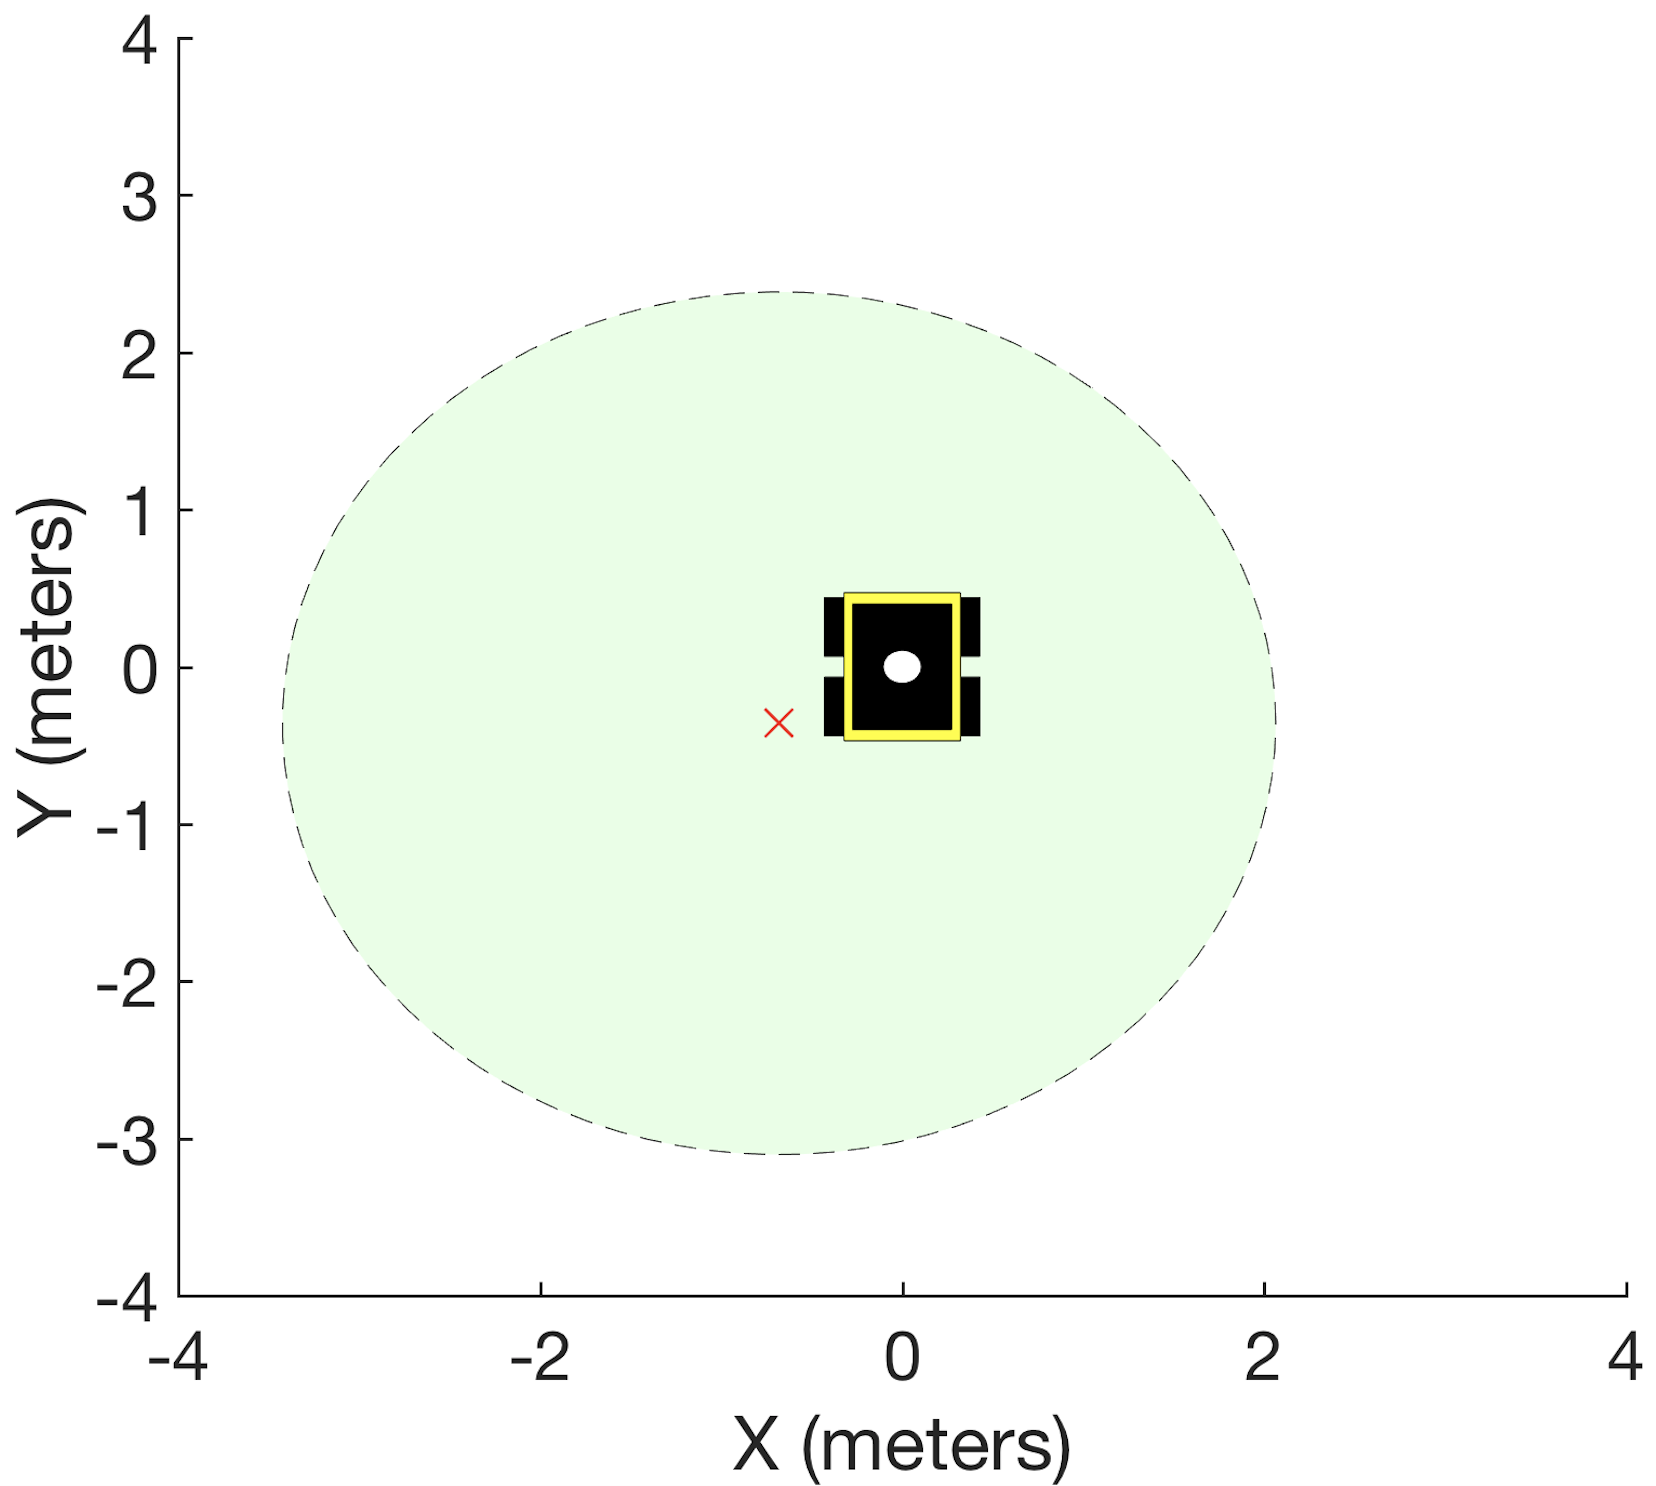
\includegraphics[width = 0.22\textwidth]{Figures/sample1.png}} &	
% \subfigure[\label{fig:5samples} ]{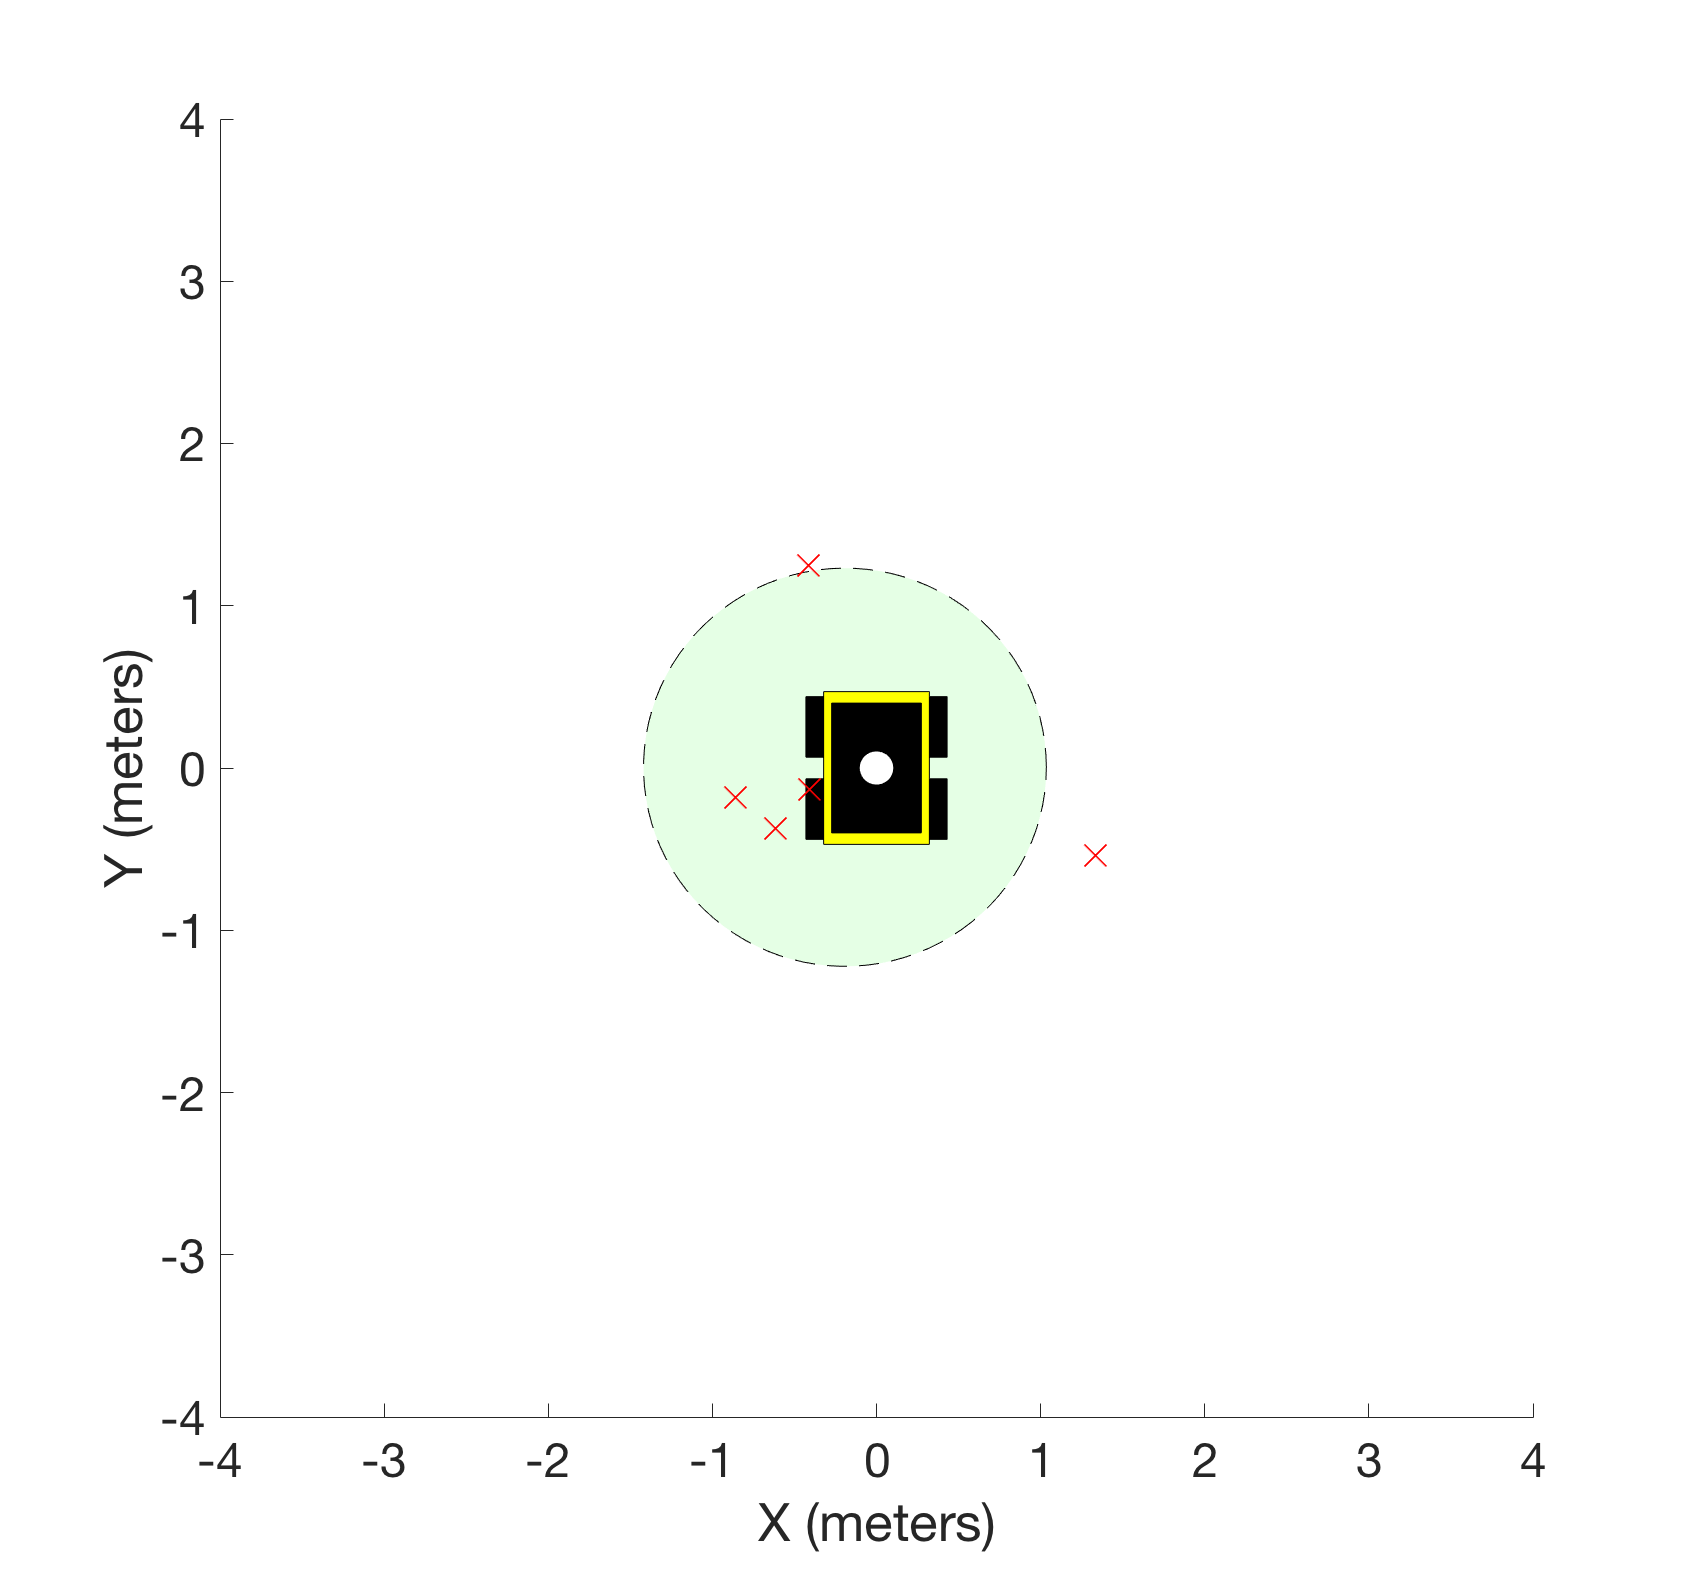
\includegraphics[width = 0.22\textwidth]{Figures/sample5.png}}
% \end{tabular}
% \caption{A comparison of the size of the estimated confidence region as the $N_e$ number of data samples grow. In \ref{fig:1sample}, the estimated confidence region with 1 data sample is not as accurate. In \ref{fig:5samples}, the $N_e$ number of samples used is five, which gives a much smaller size and more accurate confidence region.}
% \label{fig:confidence_region}
% \end{figure}

Similar to the calculation of confidence intervals \eqref{Confidence_interval}, the true mean is assumed static (i.e. is not changing over time). To take vehicle mobility into account, we propose an adapted approach to compute the confidence region using previous estimated position measurements $\bm{p}(k-i)$, where $i=1,\dots,N-1$. These $N-1$ number of previous measurements need to be represented as if they were all sampled for the current position in time $k$, creating a static set of data. Using a static set of measurements, we are able to calculate a confidence region using more than one sample to improve estimation accuracy. The $N$ position estimate samples are described in the set $\bm{P}=\begin{bmatrix} \bm{p}(k) ,\bm{p}(k-1),\dots,\bm{p}(k-N+1) \end{bmatrix} $.
%\begin{equation}
%    \bm{P}=\begin{bmatrix} \bm{p}(k) ,\bm{p}(k-1),\dots,\bm{p}(k-N+1) \end{bmatrix} 
%\end{equation}
To compute the static case, we need to translate each historic element forward with the following transformation:
	\begin{equation}
	\bm{p}^*(k-i) = \bm{p}(k-i)+\sum_{j=i}^1 v(k-j)\theta_h(k-j)t_s 
	\end{equation}
%where $i=1,\dots,N-1$. 
Translating the data coordinates into a static form creates the updated set $\bm{P}^*=\begin{bmatrix} \bm{p}^*(k) ,\bm{p}^*(k-1),\dots,\bm{p}^*(k-N+1) \end{bmatrix} $.
%\begin{equation}
%    \bm{P}^*=\begin{bmatrix} \bm{p}^*(k) ,\bm{p}^*(k-1),\dots,\bm{p}^*(k-N+1) \end{bmatrix} \nonumber
%\end{equation}
The mean of the updated set is written as $\bar{\bm{p}}^*$, which is the estimated center point used in the calculation of the confidence region. Fig. \ref{fig:pseudo_static} gives a visualization of the procedure used to translate forward position estimates and obtain a pseudo-static case during two steps.

\begin{figure}[ht!]
\vspace{1pt}
\begin{tabular}{cc}
\subfigure[\label{fig:step_one} ]{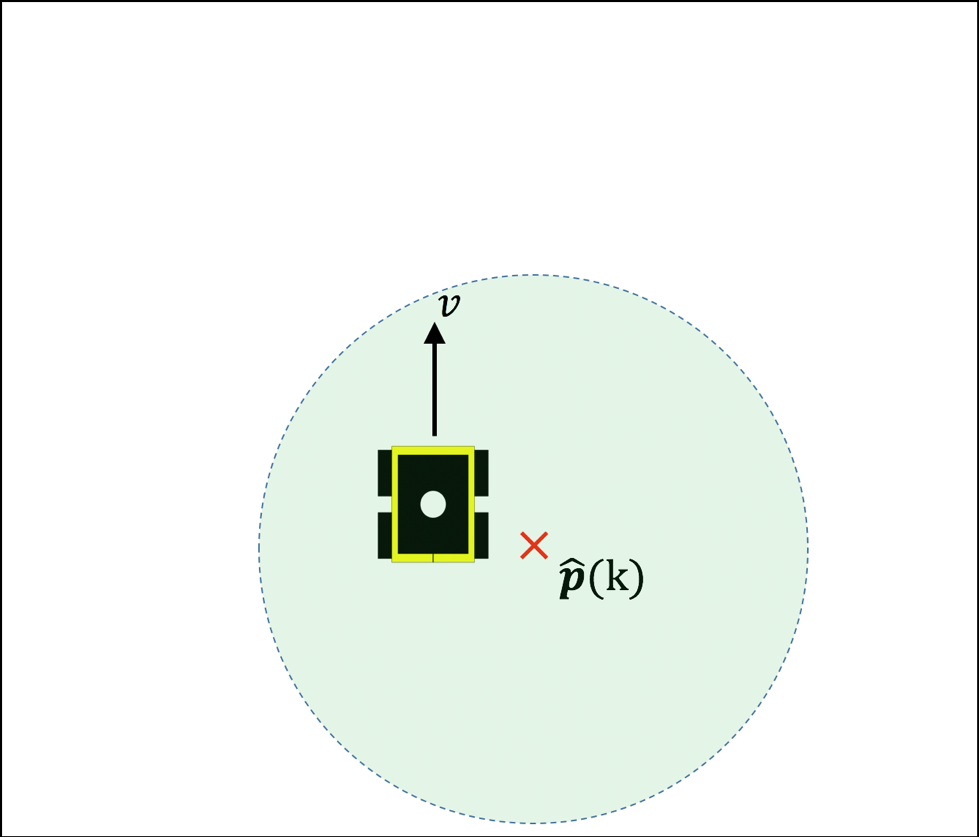
\includegraphics[width = 0.21\textwidth]{Figures/pseudo_static_left.png}} &	
\subfigure[\label{fig:step_two} ]{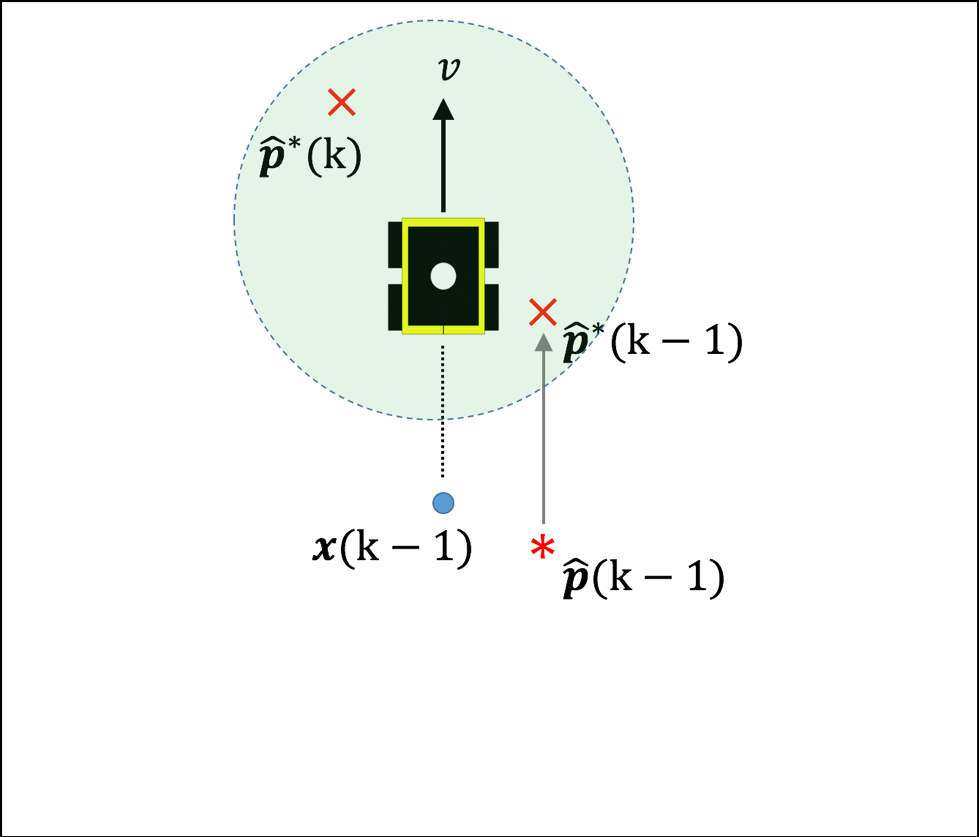
\includegraphics[width = 0.21\textwidth]{Figures/pseudo_static_right.png}}
\end{tabular}
\caption{Translation of the original position estimates $\bm{p}$ to a static case $\bm{p}^*$ as if all the position estimates were sampled from the vehicle at the current time interval $k$.}
\label{fig:pseudo_static}
\vspace{-10pt}
\end{figure}


Creating a static case with these past position data samples introduces an error while translating. Measurement uncertainty from the velocity sensor $\sigma_v$ and heading angle sensor $\sigma_h$ need to be accounted for to guarantee that the true position of the vehicle is within the estimation radial bounds. The calculation for the translation error $\epsilon_{v,\theta}$ is omitted here, but its result is included in the final calculation of the confidence region, \eqref{Confidence_region} becomes,
    \begin{equation}
    \label{Confidence_region_updated}
		C_{\bar{\bm{p}}^*|N} = \bar{\bm{p}}^* + c_p\frac{\sigma_p}{\sqrt{N}} + \epsilon_{v,\theta}
	\end{equation}
% with a radius around the center point $\bar{\bm{p}}^*$,
%     \begin{equation}
%     \label{Confidence_radius2}
% 		C_r = c_p\frac{\sigma_p}{\sqrt{N}} + \epsilon_{v,\theta}
% 	\end{equation}
that accounts for all $N-1$ translated previous data points to appear as if they all were sampled at time interval $k$.

%     \begin{align}
%     \begin{split}
% 	&\epsilon_{v,\theta}=\Big( \big[(\bar{v}^* \cos(N_{\sigma}\sigma_h) - \bar{v}) \big]^2 \\
% 	+ & \big[ (\bar{v}^* \sin(N_{\sigma}\sigma_h) - 0) \big]^2 \Big) ^{1/2} (N_e-1)
% 	\end{split}
% 	\end{align}
%     \begin{equation}
%     \label{eq:avg_vel}
%     \bar{v}=\sum_{j=0}^{N_e-1} \frac{v(k-j)}{N_e}
% 	%\bar{v}^{*}=\bar{v}(k-i_{C^{*}})+c_p\sigma_v \nonumber
% 	\end{equation}
%     \begin{equation}
%     \label{eq:avg_vel_noise}
% 	\bar{v}^{*}=\bar{v}+N_{\sigma}\sigma_v 
% 	\end{equation}
% The maximum angle error is denoted as $N_{\sigma}\sigma_h$ (i.e., the maximum uncertainty of the truncated Normal distribution) and the average velocity with and without sensor error are computed in \eqref{eq:avg_vel} and \eqref{eq:avg_vel_noise}. 

%The worst case scenario is assumed in the both the velocity and angle measurement error. Including the uncertainty due to velocity and angle measurements, the confidence region from \eqref{Confidence_region_updated} is updated to,
%     \begin{equation}
%     \label{Confidence_region_updated2}
% 		C_{\bar{\bm{p}}^*|N_e} = \bar{\bm{p}}^* + c_p\frac{\sigma_p}{\sqrt{N_e}} + \epsilon_{v,\theta}
% 	\end{equation}

\subsection{Adaptive Motion Planning}

% Thus here we are interested to compute a confidence interval around our state estimation and adapt the vehicle's motion plan if safety constraints could be violated

Using the approach just  described, we can increase confidence in the state estimation by gathering more data when necessary and guarantee safety. For example a vehicle in an open space far from obstacles, doesn't need a very accurate state estimation to guarantee safety, while the same vehicle in a cluttered environment may need more accuracy and thus more samples to precisely estimate its position.

%With uncertainty of sensor measurements, with or without a reconfigured set of sensors, there needs to be guarantees to navigate safely. As the vehicle approaches an undesired region, we need to gather more data to reduce the size of the confidence region to guarantee safety. 

To gather more data there are two options: i) to sample data faster or ii) to reduce velocity. However, sampling at a faster rate cannot be done due to physical limitations, hence adapting the velocity of the vehicle is the only way to gather more data in a shorter distance to reduce estimation uncertainties. 
%To ensure the confidence region never intersects with an undesired state (e.g., an obstacle), we update the number of data samples for better estimation while also adapting the velocity.


To update the size of the confidence region, we compute the distance $d_p$ the vehicle can travel to the next time interval $k+1$. If an undesired region is within $C_{\bar{\bm{p}}^*|N} + \Delta(k)$ at the next predicted state $\bm{p}^*(k+1)$, the next value of $N$ is computed as:
    \begin{equation}
    \label{eq:N}
	    N = round \left(c_p \frac{ \sigma_p }{ {\min \lVert \bm{p}_o - \bar{\bm{p}}^*(k+1) \rVert} -\Delta(k) } \right)^2
	\end{equation}
where $round$, rounds $N$ up to the nearest integer and $\Delta(k)$ is a boundary which represents the maximum distance the confidence region may shift as it is not always centered over the position of the vehicle.

An update of the reference velocity needs to occur when these undesired states are within the confidence region $ C_{\bar{\bm{p}}^*|N}+\Delta(k)$. Slowing down allows us to capture more previous data samples with less estimation error. 


The maximum allowable velocities are related to the distance of an undesired state to the confidence region and next estimated position in time $k+1$ are computed as:
	\begin{equation}
	\label{eq:ref_vel_options}
%	    \Tilde{r}_v(k) = \frac{d_p}{Nt_s}, \;\;\;\; \bar{r}_v(k) = \frac{\delta_{\Delta}}{t_s}
	    {r}_v^d(k) = \frac{d_p}{Nt_s}, \;\;\;\; {r}_v^{\delta}(k) = \frac{\delta_{\Delta}}{t_s}
	\end{equation}
where $d_p$ is the distance the vehicle can travel at the desired reference velocity and $\delta_{\Delta}$ is the minimum distance between an undesired state and the confidence region. Considering a worst case scenario, the minimum reference velocity is chosen to ensure a velocity to safely navigate without entering an undesired state as:
    \begin{equation}
    \label{eq:ref_vel}
        r_v(k) = \min\{{r}_v^d(k), {r}_v^{\delta}(k) \}
	\end{equation}

\begin{lemma} 
	\label{lemma_2}
Using the adaptive motion planning approach in \eqref{eq:N}, \eqref{eq:ref_vel_options}, and \eqref{eq:ref_vel}, a vehicle is guaranteed to never enter an undesired state $\bm{p}_o$ between two consecutive states $\bm{p}(k)$ and $\bm{p}(k+1)$.

\end{lemma}

\begin{proof}
With the vehicle at a state $\bm{p}(k) \neq \bm{p}_o$, there exists a reference velocity $r_v(k)\geq0$ such that next state $\bm{p}(k+1)$ will never enter an undesired state $\bm{p}_o$. Using \eqref{eq:N}, the required number of data samples are computed to guarantee the confidence region \eqref{Confidence_region_updated} at $\bm{p}(k+1)$ will never intersect with an undesired state $C_{\bar{\bm{p}}^*(k+1)|N} \cap \bm{p}_o = \emptyset$. ${r}_v^{\delta}$ in \eqref{eq:ref_vel} selects always the minimum velocity between $r_v^{d}$ and $r_v^{\delta}$. The worst case scenario happens when $r_v^{d}>r_v^{\delta}$, thus we need to guarantee that $r_v^{\delta}t_s-\bm{p}_o\geq0$ assuming that $\bm{p}\in C_{\bar{\bm{p}}}^*$ is in the closest point to $\bm{p}_o$. This constraint is true by definition since from \eqref{eq:ref_vel_options} $ {r}_v^{\delta}$ is computed considering the minimum distance $\delta_{\Delta}$ between the vehicle and the undesired state, hence proving that the reference velocity will not send the vehicle into an undesired state. 
%\begin{equation}
%\label{lemma_2_eq1}
%    C_{\bar{\bm{p}}^*(k+1)|N} \cap \bm{p}_o = \emptyset \nonumber
%\end{equation}

%By knowing $d_p$ and the confidence region \eqref{Confidence_region_updated} at time interval $k$
%
%With the knowledge of the closest distance between an undesired state $\bm{p}_o$ and confidence region \eqref{Confidence_region_updated} at time interval $k$, the reference velocity \eqref{eq:ref_vel} is computed such that the vehicle will not travel more than a distance $d_p$ to avoid the undesired state,
%\begin{equation}
%\label{lemma_2_eq2}
%    \min \lVert \bm{p}_o - C_{\bar{\bm{p}}^*(k)|N} \rVert > \frac{d_p}{N} \geq r_v(k)t_s
%  \nonumber
%\end{equation}
%proving that the reference velocity will not send the vehicle into an undesired state. 
%The system uses a closed loop controller to always converge toward the trajectory with the assumption that the trajectory never crosses through an undesired state.
\end{proof}
%	\begin{equation}
%		\Delta(k)=[v(k)]^{\delta_v}\delta
%	\end{equation}
%where $[\delta, \delta_v] \in R^{\geq0}$ are chosen values that determine the desired distance between the closest unwanted region to the estimation region as a function of velocity.




% % INSERT ALGORITHM FOR REPLANNING VELOCITY
% \begin{algorithm}
%   \caption{Adaptive Motion for Safe Navigation} 
%   \label{alg:adapt_motion} 
%     \begin{algorithmic}[1]
% 	\State Initial conditions of system: $k=0$,$\bm{x}(0)=\bm{x}_0$
% 	\State Set $r_v(0)$ to desired velocity $r_{des}$
%     \While{$1<k\leq\infty$}
%         \State \Longunderstack[l]{ Calculate $\bar{\bm{p}}^*$ then measure closest distance\\ to undesired region $\min \lVert \bm{x}_r - \bar{\bm{p}}^* \rVert$.}
%         \State Calculate radii of intervals $\varepsilon_1$ and $\varepsilon_2$ for $N$.
%         \If{ $\min \lVert \bm{x}_r - \bar{\bm{p}}^*\rVert < \varepsilon_2(k)$}
%             \State Solve for $N$ of next iteration
%             \State Update reference for velocity $r_v(k)$
%         \Else
%             \If{$\min \lVert \bm{x}_r - \bar{\bm{p}}^*\rVert < \varepsilon_2(k)$ when $N=1$}
%                 \State Solve for $N$ of next iteration
%                 \State Update reference for velocity $r_v(k)$
%             \Else
%                 \If{$r_v(k) \neq r_{des}$}
%                     \State Reference velocity $r_v(k)=r_{des}$
%                     \State $N = 1$
%                 \Else
%                     \State Reference velocity $r_v(k) = r_v(k-1)$
%                     \State $N = 1$
%                 \EndIf
%             \EndIf
%         \EndIf
%     \EndWhile
% 	\end{algorithmic}
% \end{algorithm}



\end{section} 